\documentclass[12pt]{article}

%%% R
\usepackage[utf8]{inputenc}
\usepackage[english]{babel}
\usepackage[margin=1in,top=1.5in,headsep=.5in]{geometry}
\usepackage{graphicx}
\usepackage{float} % use [H] to place figures and tables exactly where you code them.
%\usepackage{array} % to define column width in the table on the title page
\usepackage{hyperref}
    \hypersetup{
    colorlinks=true,
    linkcolor=black,
    filecolor=magenta,      
    urlcolor=cyan,
    }
    \urlstyle{same}
\usepackage{microtype} % Greatly improves general appearance of the text and reduces amount of “under-” and “overfull box” warnings that LaTeX usually reports in the compilation logs
\usepackage{fancyhdr}
%\usepackage{multicol} % Handles multicolumn documents

%%% For bibliography
\usepackage[backend=biber, style=numeric]{biblatex}
\addbibresource{refs.bib}

%%% Packages just for drafting stage
%\usepackage{todonotes} %See Todonotes documentation for usage.
%\usepackage{lipsum} %For generating dummy text to test typesetting. Lipsum package has access to 150 paragraphs of “Lorem ipsum” dummy text. \lipsum[1] will only print lorem ipsum paragraph 1. \lipsum[2-4] will print lorem ipsum paragraph 2 to 4.

%%% Configure directory location for importing sections
\usepackage{import}
\newcommand*{\sectiondir}{sections/}

%%% Headers and footers
\pagestyle{fancy}
\fancyhf{}
\lhead{}
\chead{}
\rhead{FT-IR MOP \\ August 2018 \\ Rev. No. 1}
\lfoot{}
\cfoot{Page \thepage~of~\pageref{lastpage}}
\rfoot{}

%%% Title pages
%\title{Measurement of the infrared absorption spectrum with a Fourier-transform infrared spectrometer \\does this show up anywhere? no. \#xxxx \\NRMRL/AEMD}
%\author{Emily Li}
%\date{\today}
\begin{document}
\import{\sectiondir}{titlepage.tex}
%\begin{abstract} %%% This is a simple paragraph at the beginning of the document. A brief introduction about the main subject.
%\end{abstract}
%\listoftodos \newpage %%% just for drafting stage
\tableofcontents \newpage
%\listoffigures %%% probably also just for drafting
%\newpage

%%% BEGIN MOP %%%
\section{Scope and Application}
This miscellaneous operating procedure (MOP) describes the procedure for measuring Fourier-transform infrared (FT-IR) absorbance spectra of membrane air filter samples on a FT-IR spectrometer. Light absorption measurements obtained by FT-IR can be used for a variety of applications such as quantifying the underlying composition of organic and inorganic functional groups containing molecular bonds with a dipole moment. This MOP will cover the basic procedures of the filter absorption measurement that will be common to any such application.

This MOP is intended for scientists, engineers, and technicians seeking to measure the absorption spectrum of a membrane air sampling filter. This MOP will describe the procedures necessary to make an absorption measurement from membrane air sampling filters. Sample preparation and collection procedures will be covered in separate project-specific quality assurance project plans (QAPPs).

\section{Personnel}
A table of responsible personnel is shown in Table \ref{tab:personnel}.

\begin{table}[H]
    \centering
    \begin{tabular}{l l}
         \textbf{Name} & \textbf{Role} \\
         Emily Y. Li & Analyst \\
         Michael D. Hays & Principal Investigator \\
         Richard Shores & Distributed Source \& Buildings Branch Chief\\
         Libby Nessley & Quality Assurance Manager \\
         Robert S. Wright~~~~~ & Technical Services Team \\ %that's what his title was on his memo
    \end{tabular}
    \caption{FT-IR spectrometer personnel.}
    \label{tab:personnel}
\end{table}

Due to the complexity of the FT-IR spectroscopic method, new analysts must demonstrate proficiency before performing routine analyses.  For example, a new analyst will be requested to duplicate FT-IR spectroscopic measurements already performed by an experienced analyst.

\section{Method Summary}
This method covers the procedures for measuring the absorption spectrum of a membrane air sampling filter with a TENSOR II Spectrometer (Bruker Corporation, Billerica, MA) equipped with a liquid nitrogen-cooled detector. Water vapor and $CO_2$ are purged from the sample compartment and instrument optics to minimize absorption bands of gas phase ucompounds in the aerosol spectra. 

Samples are measured in transmission-mode, where the IR beam is directed through the sample. Absorbance ($A$) can be obtained by ratioing the measured extinction of radiation through the sample ($I$) by a reference value ($I_0$, also called the ``background") and taking the negative value of their base-10 logarithm (Eqn. \ref{eqn:transabs}). The absorbance across a range of IR beam wavenumbers is an absorbance spectrum using the most recent empty chamber spectrum as a reference, collected hourly. The quality of the absorbance spectrum depends on how accurately the background reflects the conditions of the sample scan, and therefore the background is acquired regularly. The total measurement time for one filter is approximately 5 minutes.

\begin{equation}
    A = -log_{10}\frac{I}{I_0}
\label{eqn:transabs}
\end{equation}

\section{Definitions}
\begin{itemize}
    \item Measuring device: TENSOR II FT-IR Spectrometer (Bruker Corporation, Billerica, MA).
    \item Sample holder: Square stainless steel box with a slot and lid, custom-built to hold each filter sample the same distance from the source.
    \item Wavenumber: the number of waves in one centimeter. Directly proportional to and used as a measure of the specified energy of the light source, and has the units of reciprocal centimeters ($cm^{-1}$).
    \item Detector: the liquid nitrogen-cooled mid-IR detector used for FTIR measurements.
\end{itemize}
%\begin{figure}
%\begin{center}
%%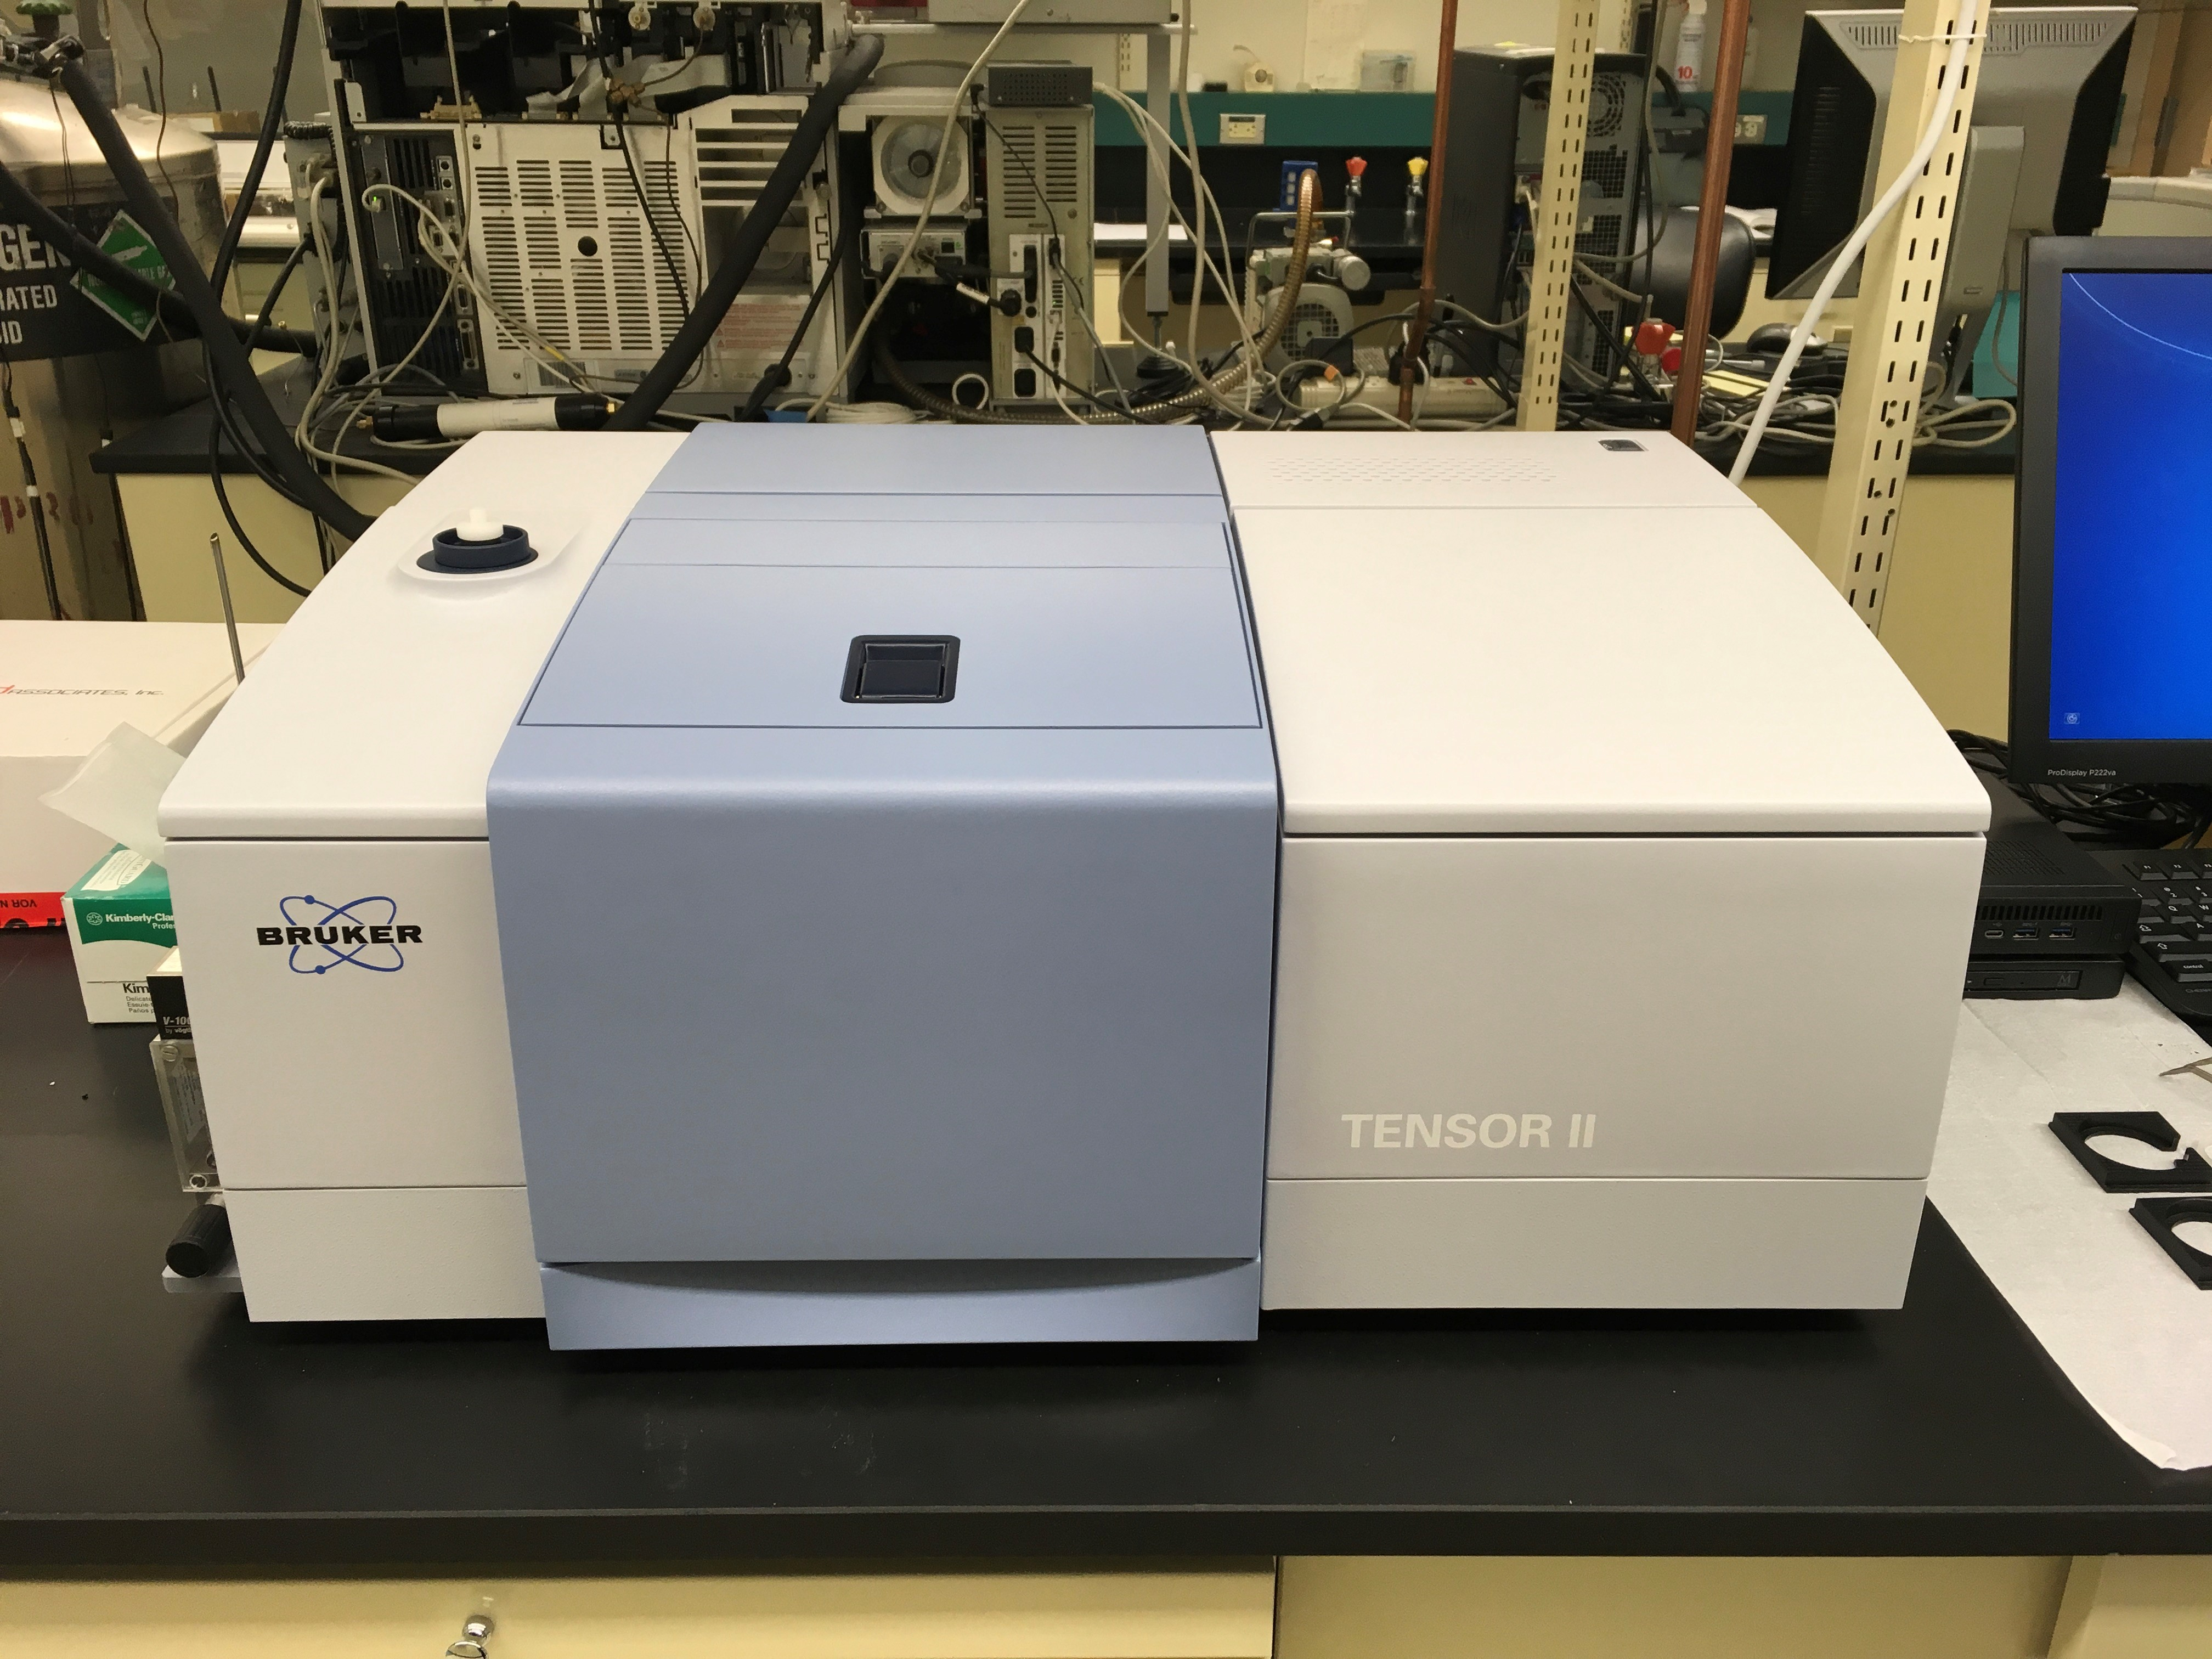
\includegraphics[width=6.5in]{TENSOR.jpg}
%\missingfigure[]{Provide a diagram of the sample holder with dimensions or a photograph of it. (Mike, the design is proprietary. Is a photograph okay?)}
%\caption{FT-IR sample holder.}
%\label{FTIRsampleholder}
%\end{center}
%\end{figure}

\section{Health and Safety Considerations}
Laboratory safety practices should be in accordance with the sample and standard laboratory practices. Gloves, lab coat, and safety glasses should be used as necessary.

Liquid nitrogen, which is a cryogenic fluid, is used when setting up the FT-IR instrument. There are two groups of safety hazards associated with cryogenic liquid nitrogen: extreme cold and asphyxiation.

The TENSOR II FT-IR spectrometer is equipped with a laser diode that is classified as a laser class 1 product\cite{Bruker1}.

Safety measures to be taken with extreme cold, asphyxiation, and laser radiation hazards are detailed in Subsections \ref{subsec:cold}-\ref{subsec:laser}.

\subsection{Extreme cold hazard}
\label{subsec:cold}
Cryogenic liquids and vapors can produce effects on skin similar to a thermal burn. Brief exposures that would not affect skin on the hands can still damage delicate tissues such as the eyes. Prolonged breathing of extremely cold air may damage the lungs. A face shield must be worn when dispensing or transporting liquid nitrogen. The face shield must be used in conjunction with safety glasses or goggles. 

Prolonged exposure of the skin or contact with cold surfaces can cause frostbite. Unprotected skin can stick to extremely cold metal, tearing the skin when pulled away. Even non-metallic materials are dangerous to touch at low temperatures. Thermally insulating gloves must be worn while handling liquid nitrogen.

When transporting liquid nitrogen, use a double-walled vessel, such as a glass dewar flask. In these vessels, the space between the two walls is a vacuum, which means a crack forming in the inner or outer wall may cause a sudden implosion. With cryogenic fluid inside, a crack may cause a sudden expansion of cryogenic gas that may explode the vessel. Handle such vessels carefully for personal safety and to prevent breakage.

\subsection{Asphyxiation hazard}
When liquid nitrogen forms a gas, the gas displaces oxygen in the air. When there is not enough oxygen, asphyxiation and death can occur. Oxygen deficiency is a serious hazard in enclosed or confined spaces. Small amounts of liquid nitrogen can evaporate into very large volumes of gas. For example, one liter of liquid nitrogen evaporates to 695 liters of nitrogen gas when warmed to room temperature ($21^\circ C$). Do not dispense liquid nitrogen in enclosed or confined spaces.

\subsection{Hazardous laser radiation}
\label{subsec:laser}
The TENSOR II spectrometer is classified by the International Electrotechnical Commission standard (IEC 60825-1:2007) as a laser class 1 product. According to this classification, laser radiation is not accessible for the user if the spectrometer is used as intended. Intended use is defined in Section 1.5 of the TENSOR II User Manual\cite{Bruker1}.

Inside the interferometer, the semiconductor vertical-cavity surface-emitting laser (VCSEL) diode emits invisible light with a wavelength of 850 nm at power output 2 mW. IEC 60825-1:2007 classifies this laser component as laser class 3B\cite{Bruker1}.

According to the TENSOR II User Manual, there may be potential risk of exposure to laser class 3B radiation in the cases of damaged spectrometer housing or unauthorized removal of the laser safety cover. \textbf{In these cases, switch off the spectrometer immediately.} Avoid any eye exposure to the laser radiation, and keep in mind that this laser radiation is invisible. The TENSOR II FT-IR power switch is located in the back of the spectrometer (see Figure \ref{FTIRswitch} on page \pageref{FTIRswitch}).

\section{Limits of Application}
Ambient temperature must be between 18$^\circ C$ and 35$^\circ C$ at a non-condensing humidity ($\le 80\%$ relative humidity). See the TENSOR II User Manual\cite{Bruker1} for more site requirements. 

%%% These were large sections. It's easier to edit them in separate files, which are in the sections folder. That way, if rearrangement is needed, you only have to rearrange these import commands.
\import{\sectiondir}{equipment.tex}
\import{\sectiondir}{measurement.tex}
\import{\sectiondir}{QC.tex}

\printbibliography
\label{lastpage} %%% Used to \ref the total number of pages in the footer.
\end{document}